\documentclass[10pt]{iopart}
\usepackage{graphicx}
\usepackage{iopams}

\begin{document}

\title[Algorithm suitability for photonic continuous-variable hardware]{Algorithm suitability for photonic continuous-variable
quantum computers: a comparative resource and noise-robustness study}

\author{Hikaru Wakaura$^{1}$ and Taiki Tanimae$^{1}$}
\address{$^{1}$ QIRI (Quantum Integrated Research Institute Inc.),
1--16--3 Akasaka, Minato-ku, Tokyo 107--0061, Japan}
\ead{h.wakaura@deeptell.jp} 

\begin{abstract} 
Photonic continuous-variable (CV) processors are a leading route to scalable
quantum computing, yet the fault-tolerance cost of an algorithm depends on its
use of controlled unitaries, non-Gaussian gates, and depth. We port four
algorithms---control-free phase estimation, randomized product formulas,
quantum Kolmogorov--Arnold networks, and Regev factoring---to a common CV model
and compare them under photon loss and Gaussian displacement with
Gottesman--Kitaev--Preskill (GKP) correction. Control-free phase estimation is
the most noise-robust, needing no controlled unitaries and, for quadratic
Hamiltonians, no non-Gaussian gates. Correction helps only above the
finite-squeezing floor; a noise- versus systematic-limited dichotomy predicts
which algorithms benefit.  
\end{abstract}
   
\maketitle
\ioptwocol 
  
Photonic continuous-variable (CV) architectures encode information in the
quadratures of bosonic modes and support deterministic, room-temperature
generation of large cluster states~\cite{Lloyd1999,Menicucci2014,Larsen2019,
Asavanant2019,Madsen2022}, making them a leading candidate for scalable
fault-tolerant quantum computing. Fault tolerance is supplied by bosonic codes,
most prominently the Gottesman--Kitaev--Preskill (GKP) code~\cite{GKP2001},
whose overhead is set by the achievable squeezing and the number of
non-Gaussian resource states consumed~\cite{Fukui2018,Bourassa2021,Tzitrin2021,
Noh2020}. A defining constraint is that Gaussian errors cannot be corrected by
Gaussian operations~\cite{Niset2009}, so non-Gaussian resources are mandatory.

Different algorithms place very different demands on this substrate: some
require controlled unitaries, which are costly on CV hardware because they need
a clean control mode and high non-Gaussianity; some are dominated by
non-Gaussian gate count; some by circuit depth. A unified comparison of which
algorithm classes are intrinsically robust on CV hardware, and of how much GKP
correction improves them, has been lacking. Here we port four representative
algorithms to a common CV model, compare them under a shared photon-loss and
displacement channel, and identify a finite-squeezing threshold and a
noise-versus-systematic-limited dichotomy that together predict robustness and
correction gain. We are explicit about which results are exact, which are
validated model surrogates, and which are extrapolations.

We map each algorithm onto bosonic modes encoded, where fault tolerance is
required, in GKP qubits. Gaussian operations (interferometers, squeezers, phase
rotations) are treated as inexpensive; non-Gaussian gates (cubic-phase, GKP
magic states) are the costly resource, analogous to the $T$-count of
discrete-variable (DV) circuits.

The four algorithms span the axes that govern CV cost. (i)~Control-free phase
estimation~\cite{Clinton2026} acquires the time series
$f(t)=\langle\psi|e^{iHt}|\psi\rangle$ without controlled unitaries and recovers
the spectrum by reference-eigenstate holographic phase retrieval; for quadratic
$H$, $e^{iHt}$ is purely Gaussian. (ii)~Randomized product formulas
(qDRIFT)~\cite{Campbell2019,Chen2021} approximate $e^{-iHt}$ by
importance-sampled bosonic terms with a step count independent of the number of
terms. (iii)~Quantum Kolmogorov--Arnold
networks~\cite{Ivashkov2024,Liu2024} realize quantum singular value
transformation~\cite{Low2017,Gilyen2019,Rossi2022}, with Chebyshev response
$T_r(x)=\cos(r\arccos x)$ that maps to phase-space rotations. (iv)~Regev factoring~\cite{Regev2023,Shor1997}
prepares a discrete-Gaussian GKP comb, applies a mode-wise CV quantum Fourier
transform, and runs modular exponentiation on GKP qubits.

Per noise-exposed operation we apply photon loss (transmissivity $\eta$) as an
exact Fock-space Kraus channel,
$E_l=\sqrt{(1-\eta)^l/l!}\,\eta^{\hat n/2}a^l$, and Gaussian displacement
(standard deviation $\sigma_d$) as an exact unitary kick; the dynamical
evolution is simulated exactly in truncated Fock space. GKP correction reduces
the residual to
\begin{equation}
\sigma_{\rm corr}^2=(1-p_L)\Delta^2+p_L\,\sigma_{\rm phys}^2,
\label{eq:corr}
\end{equation}
where $\sigma_{\rm phys}^2=\sigma_d^2+(1-\eta)/2$, $\Delta(\mathrm{dB})$ is the
finite-squeezing peak width, and $p_L$ is the single-round GKP logical error
rate from the standard shift-error model,
$p_L=1-[\mathrm{erf}(\frac{\sqrt\pi/2}{\sqrt2\,\sigma_{\rm eff}})]^{2}$ with
$\sigma_{\rm eff}^2=\sigma_{\rm phys}^2+\Delta^2$. We validate
Eq.~(\ref{eq:corr}) against an explicit Glancy--Knill error-correction Monte
Carlo~\cite{Glancy2006}: the analytic $p_L$ reproduces the protocol to within
$3\times10^{-4}$ absolute, the post-correction residual equals the floor
($\sigma_{\rm res}/\Delta=1.00$), and the surrogate matches the explicit
two-channel model to within $0.1\%$. Stochastic quantities use ten random seeds
with $95\%$ confidence intervals; all scripts and data reproduce every figure.

\emph{Robustness.} Under increasing displacement, control-free phase estimation
keeps its error near the clean floor ($1.8\times10^{-3}$) up to
$\sigma\!\approx\!0.20$, whereas qDRIFT, the network model, and Regev are
already degraded by $\sigma\!\approx\!0.05$. This ordering follows from the
absence of controlled unitaries and, for quadratic $H$, non-Gaussian gates in
phase estimation.

\emph{Floor crossing.} From Eq.~(\ref{eq:corr}),
$\sigma_{\rm corr}<\sigma_{\rm phys}$ if and only if
$\sigma_{\rm phys}>\Delta$, because $\sigma_{\rm corr}^2-\sigma_{\rm phys}^2
=(1-p_L)(\Delta^2-\sigma_{\rm phys}^2)$ and $1-p_L>0$. GKP correction therefore
reduces error only when the physical noise exceeds the finite-squeezing floor
$\Delta(\mathrm{dB})$, and is counterproductive below it. Figure~\ref{fig:sweep}
maps the improvement factor versus squeezing at a fixed operating point
($\sigma_d=0.10$, loss $0.15$); the floor crossing is evident, and at $18$~dB
the factors are $1.1$ (phase estimation), $1.4$ (qDRIFT), $2.5$ (network), and
$2.7$ (Regev).

\emph{Noise- versus systematic-limited dichotomy (empirical observation).}
The error of each algorithm is well described by an envelope
$\max(F,\,c\sqrt{D}\,\sigma)$, with an algorithm-specific systematic floor $F$
(e.g.\ finite acquisition window for phase estimation), depth $D$, per-step
residual $\sigma$, and an algorithm-dependent constant $c$ fit from the
clean-noise sweep. In the noise-limited regime ($c\sqrt D\sigma>F$) the GKP
gain is $\approx\sigma_{\rm phys}/\sigma_{\rm corr}>1$, realised most strongly
by deep, noise-sensitive algorithms (Regev and the network model). In the
systematic-limited regime ($F>c\sqrt D\sigma$) corrected and uncorrected
errors coincide at $F$ and the factor tends to unity. Control-free phase
estimation is systematic-limited up to $\sigma\!\approx\!0.2$: it is the most
accurate yet shows the smallest improvement factor, reconciling ``most robust''
with ``smallest correction gain''. Least-squares fits of
$\mathrm{err}^2=F^2+c_{\rm eff}^2\,\sigma_{\rm phys}^2$ over the five-point loss
sweep (Table~\ref{tab:fit}) give $R^2\!\ge\!0.89$ and locate each algorithm in
its regime: $F$ dominates for phase estimation (its systematic FFT floor) and
sets the qDRIFT algorithmic floor (finite-$N$ Trotter-like error), while
$c_{\rm eff}\,\sigma_{\rm phys}$ dominates for the network model and Regev.

\begin{table}[t]
\caption{Empirical fits of the dichotomy envelope
$\mathrm{err}^2=F^2+c_{\rm eff}^2\sigma_{\rm phys}^2$ over the loss sweep
($\sigma_d=0.10$, loss $\in\{0,0.02,0.05,0.10,0.20\}$). Units of $F$ and
$c_{\rm eff}$ are each algorithm's natural error unit.}
\label{tab:fit}
\begin{tabular}{lccc}
\br
algorithm & $F$ & $c_{\rm eff}$ & $R^2$ \\
\mr
phase estimation & $3.0\times10^{-3}$ & $3.1\times10^{-3}$ & 0.99 \\
qDRIFT & 0.47 & 1.5 & 0.89 \\
network model & 0 & 0.96 & 0.95 \\
Regev & 21 & $1.9\times10^{2}$ & 0.97 \\
\br
\end{tabular}
\end{table}

\emph{Phase diagram and ensembles.} Figure~\ref{fig:phase} extends the floor
crossing across the $(\sigma_d,\mathrm{loss})$ plane: the helpful region is
broad for deep algorithms and narrow for phase estimation. Over ensembles of
twenty random Hamiltonians, qDRIFT's clean channel error is $0.17\pm0.07$, and
control-free phase estimation recovers peak frequencies to median
$1.7\times10^{-3}$ with full success provided the holographic reference beam is
sufficiently strong---an explicit applicability condition.

\emph{Generalization to non-Gaussian Hamiltonians.} For
$H=\omega\hat n+\frac{g}{2}(a^2+a^{\dagger2})+\chi\hat n^2+\kappa x^3$,
holographic recovery returns the absolute spectrum with error
$\approx1.3$--$1.7\times10^{-3}$ that is independent of the non-Gaussian
fraction (from $0$ to $0.83$), while the controlled-unitary count remains zero.
The control-free property is thus a feature of the protocol, not of $H$ being
quadratic; non-Gaussian $H$ only adds the cost of a Trotterized $e^{iHt}$.

\emph{Discrete-variable baseline.} Against a rotated surface code at physical
error $3\times10^{-3}$, reaching logical error $10^{-6}$ needs distance $17$,
i.e.\ $577$ physical qubits per logical qubit; a single-round GKP mode at
$\sigma_{\rm phys}=0.10$ needs $\approx14$~dB, and floors above $10^{-6}$ for
$\sigma_{\rm phys}\gtrsim0.2$, requiring concatenation~\cite{Fowler2012,
Vuillot2019}. Structurally, a spectroscopy task ($10$ readout bits, $8$ system
qubits, Trotter depth $50$) costs $1023$ controlled evolutions and a $T$-count
$\sim2\times10^{7}$ in DV phase estimation, versus zero controlled unitaries and
zero non-Gaussian gates in the control-free CV protocol for quadratic $H$. The
CV advantage is structural---Gaussian operations are free---rather than a
threshold effect.

\emph{Unit-independent ranking.} Mapping each error to a dimensionless
infidelity by a monotone soft-saturating transform
$I=\mathrm{err}/(\mathrm{err}+s)$ with task-failure scale $s$ preserves the
ordering $I_{\rm PE}=0.003 < I_{\rm net}=0.25 < I_{\rm qDRIFT}=0.40
< I_{\rm Regev}=0.98$; the ordering is invariant when every $s$ varies over
$[0.5,2]\times$ its nominal value.

\emph{Regev squeezing scaling.} With $R=e^{\Theta(\sqrt n)}$ and dual tolerance
$\delta=\sqrt d/(\sqrt2 R)$, the comb readout constraint
$\sigma_{\rm cv}=\Delta/\sqrt\pi\le\delta$ gives
$\mathrm{dB}\ge10\log_{10}(R^2/\pi d)=\Theta(\sqrt n)$. The unrescaled comb
therefore demands squeezing growing as $\sqrt n$, prohibitive at cryptographic
sizes; we present Regev as a worked correctness check and a cautionary resource
case rather than a practical CV factoring route.

The findings cohere into a quantitative selection rule for CV hardware: minimize
controlled unitaries, non-Gaussian gate density, and depth. Control-free phase
estimation minimizes all three and is the most robust; GKP correction repays its
squeezing cost only above the finite-squeezing floor and in proportion to how
noise-limited an algorithm is; and CV-native cheapness of state preparation and
Fourier transforms does not rescue a depth- and readout-heavy algorithm such as
Regev. These criteria are model-level: the dynamical channels are exact, the GKP
correction is a surrogate validated to $\le0.1\%$ against an explicit
error-correction protocol but not a full Fock-space circuit with
loss-correcting amplification, and instances are modest in size. The natural
experimental target is a GKP-encoded photonic cluster-state processor at
$10$--$15$~dB squeezing, where the floor crossing and the
phase-estimation-versus-deep-algorithm dichotomy are directly testable;
control-free spectroscopy of a small bosonic or Fermi--Hubbard Hamiltonian is
the most accessible first demonstration.

The scripts and numerical results that reproduce all figures and tables are
available from the authors on reasonable request.

\ack
The authors thank colleagues at QIRI for discussions.

\begin{figure}[t]
\centering
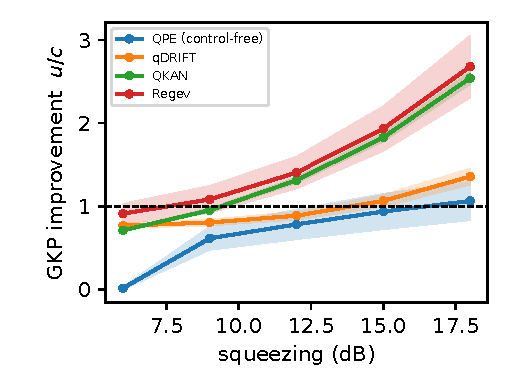
\includegraphics[width=\columnwidth]{fig_squeeze_sweep.pdf}
\caption{GKP improvement factor versus squeezing at $\sigma_d=0.10$, loss
$0.15$; shaded bands are $95\%$ confidence intervals over ten seeds. The
crossing of unity marks the finite-squeezing floor.}
\label{fig:sweep}
\end{figure}

\begin{figure*}[t]
\centering
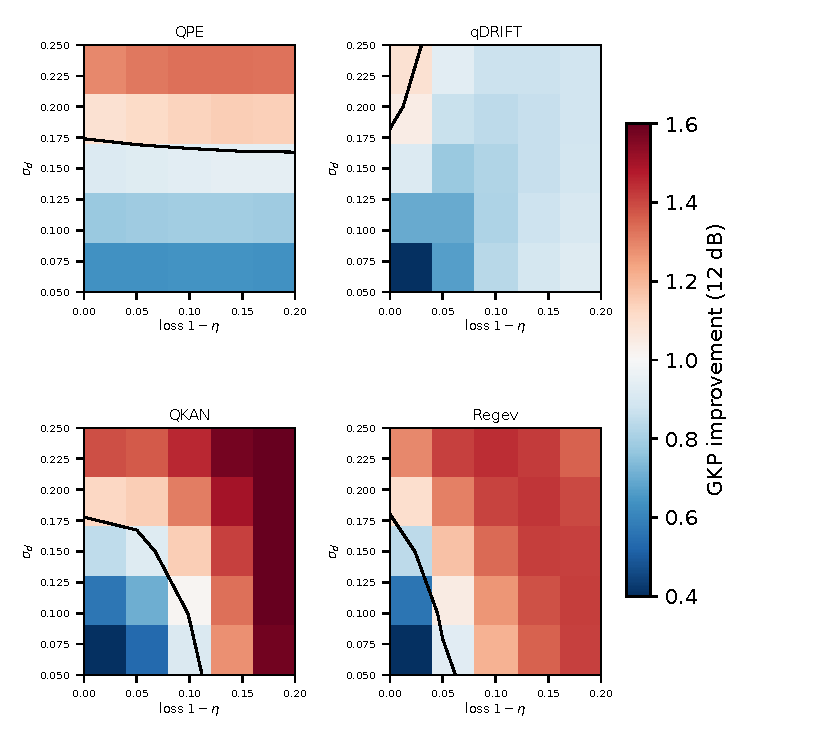
\includegraphics[width=0.7\textwidth]{fig_phase_diagram.pdf}
\caption{GKP improvement factor ($12$~dB) over the
$(\sigma_d,\mathrm{loss})$ plane; the black contour marks the floor crossing
(factor unity). Blue: correction helps; red: counterproductive.}
\label{fig:phase}
\end{figure*}

\section*{References}
\begin{thebibliography}{40}
\bibitem{Lloyd1999} Lloyd S and Braunstein S L 1999 {\it Phys. Rev. Lett.}
{\bf 82} 1784
\bibitem{Menicucci2014} Menicucci N C 2014 {\it Phys. Rev. Lett.} {\bf 112}
120504
\bibitem{Larsen2019} Larsen M V, Guo X, Breum C R, Neergaard-Nielsen J S and
Andersen U L 2019 {\it Science} {\bf 366} 369
\bibitem{Asavanant2019} Asavanant W {\it et al.} 2019 {\it Science} {\bf 366}
373
\bibitem{Madsen2022} Madsen L S {\it et al.} 2022 {\it Nature} {\bf 606} 75
\bibitem{GKP2001} Gottesman D, Kitaev A and Preskill J 2001 {\it Phys. Rev. A}
{\bf 64} 012310
\bibitem{Fukui2018} Fukui K, Tomita A, Okamoto A and Fujii K 2018 {\it Phys.
Rev. X} {\bf 8} 021054
\bibitem{Bourassa2021} Bourassa J E {\it et al.} 2021 {\it Quantum} {\bf 5} 392
\bibitem{Tzitrin2021} Tzitrin I {\it et al.} 2021 {\it Phys. Rev. X Quantum}
{\bf 2} 040353
\bibitem{Noh2020} Noh K and Chamberland C 2020 {\it Phys. Rev. A} {\bf 101}
012316
\bibitem{Niset2009} Niset J, Fiur\'a\v{s}ek J and Cerf N J 2009 {\it Phys. Rev.
Lett.} {\bf 102} 120501
\bibitem{Clinton2026} Clinton L, Cubitt T S, Garcia-Patron R, Montanaro A,
Stanisic S and Stroeks M 2026 {\it Phys. Rev. X Quantum} {\bf 7} 010345
\bibitem{Campbell2019} Campbell E 2019 {\it Phys. Rev. Lett.} {\bf 123} 070503
\bibitem{Chen2021} Chen C-F, Huang H-Y, Kueng R and Tropp J A 2021 {\it Phys.
Rev. X Quantum} {\bf 2} 040305
\bibitem{Ivashkov2024} Ivashkov P, Huang P-W, Koor K, Pira L and Rebentrost P
2024 {\it arXiv:}2410.04435
\bibitem{Liu2024} Liu Z {\it et al.} 2024 {\it arXiv:}2404.19756
\bibitem{Low2017} Low G H and Chuang I L 2017 {\it Phys. Rev. Lett.} {\bf 118}
010501
\bibitem{Gilyen2019} Gily\'en A, Su Y, Low G H and Wiebe N 2019 {\it Proc. 51st
ACM STOC} 193
\bibitem{Rossi2022} Rossi Z M and Chuang I L 2022 {\it Quantum} {\bf 6} 811
\bibitem{Regev2023} Regev O 2023 {\it arXiv:}2308.06572
\bibitem{Shor1997} Shor P W 1997 {\it SIAM J. Comput.} {\bf 26} 1484
\bibitem{Glancy2006} Glancy S and Knill E 2006 {\it Phys. Rev. A} {\bf 73}
012325
\bibitem{Fowler2012} Fowler A G, Mariantoni M, Martinis J M and Cleland A N
2012 {\it Phys. Rev. A} {\bf 86} 032324
\bibitem{Vuillot2019} Vuillot C, Asasi H, Wang Y, Pryadko L P and Terhal B M
2019 {\it Phys. Rev. A} {\bf 99} 032344
\bibitem{Braunstein2005} Braunstein S L and van Loock P 2005 {\it Rev. Mod.
Phys.} {\bf 77} 513
\bibitem{Weedbrook2012} Weedbrook C {\it et al.} 2012 {\it Rev. Mod. Phys.}
{\bf 84} 621
\bibitem{Kitaev1995} Kitaev A Y 1995 {\it arXiv:}quant-ph/9511026
\bibitem{Albert2018} Albert V V {\it et al.} 2018 {\it Phys. Rev. A} {\bf 97}
032346
\bibitem{Walshe2020} Walshe B W, Baragiola B Q, Alexander R N and Menicucci N C
2020 {\it Phys. Rev. A} {\bf 102} 062411
\bibitem{Terhal2020} Terhal B M, Conrad J and Vuillot C 2020 {\it Quantum Sci.
Technol.} {\bf 5} 043001
\end{thebibliography}

\end{document}
